\chapter{Partial Differential Equations I: Parabolic Equations}\label{ch:pde-parabolic}

In Chapters \ref{ch:ode1}-\ref{ch:ode3}, we determined functions of a single variable, such as velocity as a function of time, with ordinary differential equations.  However, many physical quantities depend on more than one variables. For example, the particle density in the three-dimensional space depends on three coordinates $x$, $y$, and $z$. Electric field $\vb{E}(x,t)$ is another example, which depend on space-time coordinates $x$ and $t$, .  Equations which determine functions of multi-dimensional variables are known as partial differential equation (PDE).  Perhaps, you already encounter such equations in other physics courses.  Diffusion equation, Maxwell equations, and Schr\"{o}dinger equation are all PDE.

PDE is both mathematically and computationally more challenging than ODE.  One numerical method that works well for one type of PDE may fail for another type of PDE. From mathematical point of view, there are three different types of PDE for a second-order PDE with two-variable function $F(x,y)$.  Its general form can be written as
\begin{equation}\label{eq:general-pde-2nd}
	a \pdv[2]{F}{x}+ b \pdv{F}{x}{y} + c \pdv[2]{F}{y} + d \pdv{F}{x} + e \pdv{F}{y} + f F + g = 0
\end{equation}
where coefficients $a$ through $g$ are constant.  The variables $x$ and $y$ are not necessarily indicating spacial coordinates.  One of them can be time. When $b^2-4 a c = 0$, the PDE is said to be \textit{parabolic}.  Similarly the PDE is \textit{hyperbolic} for $b^2 - 4 a c>0$, and \textit{elliptic} for $b^2-4 a c <0$.   Various numerical methods have been developed but they are suitable usually only for one type of PDE and unfortunately there is no single method that works for all three types.

Parabolic equations popular in physics are heat equation for temperature $T(x,t)$
\begin{equation}\label{eq:heat-eq}
	\pdv{t} T(x,t) = \kappa \pdv[2]{x} T(x,t)
\end{equation}
and diffusion equation for particle density $\rho(x,t)$
\begin{equation}\label{eq:diffusion}
	\pdv{t} \rho(x,t) = D \pdv[2]{x} \rho(x,t). 
\end{equation}
The thermal diffusion coefficient $\kappa$ and particle diffusion constant $D$ are both positive. Clearly these two equations are mathematically identical. Letting $y=t$ and $b=c=d=f=g=0$ in Eq. \eqref{eq:general-pde-2nd}, we obtain these two equations.   Since $b^2-4 a c=0$, they are parabolic.  

Schr\"{o}dinger equation
\begin{equation}
	i \hbar \pdv{t} \psi(x,t) = -\frac{\hbar^2}{2m} \pdv[2]{x} \psi(x,t) + V(x) \psi(x,t)
\end{equation}
is slightly different  from the previous two equations ($f \ne 0$ and $e$ is pure imaginary) but it is another example of parabolic PDE.

When $a c <0$ and all other coefficients vanish,  Eq. \eqref{eq:general-pde-2nd} becomes wave equation
\begin{equation}\label{eq:wave-eq}
	\pdv[2]{t}\phi(x,t) = v^2 \pdv[2]{x} \phi(x,t)
\end{equation} 
where $v$ is the velocity of wave.  In this expression $a=v^2$ and $c=-1$ and thus it is an example of hyperbolic equation.

If $a=c=1$ (thus $a c >0$),  and all other coefficients vanish, Eq. \eqref{eq:general-pde-2nd} leads to Laplace's equation
\begin{equation}\label{eq:laplace-eq}
	\pdv[2]{x} \phi(x,y) + \pdv[2]{y} \phi(x,y) = 0
\end{equation}
which is an example of elliptic PDE.  The Laplace's equation is one of the most important equations in physics and appears in many fields of physics, including, electromagnetism, fluid dynamics, thermodynamics, ...
When an inhomogeneous term is added to the Laplace equation, we have Poisson's equation
\begin{equation}\label{eq:poisson-eq}
	\pdv[2]{x} \phi(x,y) + \pdv[2]{y} \phi(x,y) = -\frac{1}{\epsilon_0} \rho(x,y)
\end{equation}
where $\phi(x,y)$ and $\rho(x,y)$ are the electrostatic potential and the charge density, respectively.
This equation is also a family of elliptic PDE.

In the present chapter we focus on parabolic equations such as diffusion/heat equations and Sch\''{o}dinfer equations.  In the next chapter, the wave equation is discussed  as an example of hyperbolic equation.  The elliptic equation
is investigated in the following chapter using Laplace's/Poisson's equations as example.


\section{Diffusion Equation}

To begin with, we look for a numerical method for a simple diffusion equation \eqref{eq:diffusion-eq}.  While the development of numerical algorithms is purely mathematical procedure, actually consideration of physical processes described by the equation helps to find a good numerical approach.   Let us consider a free diffusion of a particle.  How fast does the particle diffuses from $x_0$ to another position $x_1$?  The mean square displacement $\expval{(x_1-x_0)^2}$ is known to be proportional to time, or more precisely $\expval{(x_1-x_0)^2}=2D t$ where $D$ is the diffusion constant.   This means that the typical time to travel over the distance $L$ is given by 
\begin{equation}\label{eq:fast-passage-time}
	\tau \approx \displaystyle \frac{L^2}{2D}.
\end{equation}
The important thing is that time scale of the process $\tau$ is related to the spacial scale $L$.   Any numerical method must be consistent with this physical condition.

Next we derive the diffusion equation.  The Fick's law tells that the flux of the particles is given by
\begin{equation}\label{eq:ficks-law}
	j(x,t) = - D \pdv{x} \rho(x,t) 
\end{equation}
Substituting this flux into the continuity equation
\begin{equation}\label{eq:continuity-eq}
	\pdv{t} \rho(x,t) + \pdv{x} j(x,t) = 0
\end{equation}
we obtain the diffusion equation \eqref{eq:diffusion-eq}.   The Fick's law \eqref{eq:ficks-law} is essential when we construct boundary condition.


\section{Boundary Conditions}

\begin{figure}
\centering
\includegraphics[width=3in]{13.pde1/boundary_condition.pdf}
\caption{Three different types of boundary conditions for diffusion equations.  (a) The particle is reflected by the wall [Neumann boundary].  (b) The particle is perfectly absorbed on the wall [Dirichlet boundary].  (c) Some particles are reflected and others absorbed on the wall with a transition rate $k_\text{on}$.  The particles on the wall can desorb with a transition rate $k_\text{off}$.  This situation can be dealt with the Robin boundary condition.}
\label{fig:boundary_condition}
\end{figure}

The parabolic PDEs common in physics has the first order derivative with respect to time.
Therefore, we need only one boundary condition for time (initial condition)
\begin{equation}\label{eq:pde_initial_condition}
f(x,t_0) = g(x)
\end{equation}
where $t_0$ is the starting time.  The initial function $g(x)$ must satisfy the boundary condition for $x$ which we discuss next.

The derivative with respect to the spacial coordinates is second order and thus we need two boundary conditions.
What happens on the boundary is not determined by the PDE itself.  Separate physical processes on the boundary determine the boundary conditions.
There are many different types of boundary conditions depending on the physical situations. Among them, four types of boundary conditions are common in physics.  We use the diffusion equation (\ref{eq:diffusion}) as example.

When particles diffusing in a container reach the wall, four different kinds of boundary conditions are commonly used in physics .
In one case, particles which hit the wall are perfectly reflected back from the wall.  The particle flux going to the wall and the flux coming from the wall must be canceled out.  Hence, the net flux at the boundary must vanish.\footnote{Vanishing flux does not mean that nothing is moving.  It simply means that the number of particles moving to the left and to the right is equal on average.}  When the particles are reflected back at $x=a$, $j(a,t)=0$.  Based on the Fick's law \eqref{eq:ficks-law}, this condition implies that
\begin{equation}\label{eq:pde_neumann_boundary}
j(x=a,t)=\eval{\pdv{x} \rho(x,t)}_{x=a} = 0
\end{equation}
which is the \textit{reflective} boundary condition (also known as no-flux condition).  In mathematics, the boundary condition given by the derivative is known as Neumann boundary condition.  Note that the number of particles conserves in this boundary condition. 

In another scenario, the particles are absorbed on the wall and do not come back to the system.  Since the particles disappear at the boundary, the boundary condition is simply
\begin{equation}\label{eq:pde_dirichlet_boundary}
\rho(a,t)=0.
\end{equation}
This is the \textit{absorbing} boundary condition.  In mathematics, this is known as 
Dirichlet boundary condition.  The number of particles in the system decreases with this boundary condition.

The third possibility corresponds to the situation between the reflective and absorbing boundary conditions.  Th particles is partly absorbed with a certain rate $k_\text{on}$.   The particles absorbed on the wall desorbe from the wall with a different rate $k_\text{off}$.  The particle flux at the boundary is now defined by
\begin{equation}
D \eval{\pdv{x} \rho(x,t)}_{x=a} = k_\text{on}\, \rho(a,t) - k_\text{off}\, \sigma(t)
\end{equation} 
where $\sigma(t)$ is the number density of the particle on the wall and it satisfies the following ODE
\begin{equation}
\dv{t} \sigma(t) = k_\text{on}\, \rho(a,t) - k_\text{off}\, \sigma(t).
\end{equation}
In mathematics, the boundary condition given by
\begin{equation}\label{eq:pde_robin_boundary}
\alpha f(a,t) + \beta \eval{\pdv{x} f(x,t) }_a = g(t)
\end{equation}
is known as the Robin boundary condition.

We need the boundary condition at two different boundaries.  We don't have to use the same type of boundary conditions.  We can use one of the three types at one boundary and another type at the other boundary.  Sometime, this type of setting is called mixed boundary value problem.

Finally, we consider a system has ''no boundary''.  Consider a field $F(\rho,\theta)$ on two-dimensional space expressed with polar coordinates; i.e., radial coordinate $\rho$ and angular coordinate $\theta$.   The radial coordinate $\rho$ is defined in $[0,\infty)$ and thus regular boundary conditions are usually specified at $\rho=0$ and $\infty$.  However, the angular coordinate $\theta$ defined in $[0, 2\pi)$ does not have a boundary since $\theta=0$ and $\theta=2 \pi$ correspond to the same point on the space.  Hence, we have $F(\rho,0)=F(\rho,2\pi), \, \forall \rho$.
Instead of limiting $\theta$ in $[0, 2\pi)$,  we often use $\theta \in \mathbb{R}$ and require 
\[
F(\rho,\theta+2\pi) = F(\rho,\theta),\quad \forall \theta  \in \mathbb{R}.
\]
Then, $F$ is a periodic function with respect to $\theta$.  This is a kind of ''boundary condition'' called periodic boundary condition.

There are other cases where the periodic boundary is used.  For example,
consider an infinitely extended system filled with infinite number of particles. Since computers cannot deal with infinity, we limit the size of the system. For example, we consider only the regions between $x=-L/2$ and $x=L/2$.  However, there is no wall at the boundary.
A common trick is to use a periodic boundary condition. We assume that the system of size $L$ repeats infinitely many times by using the condition
\begin{equation}
F(x+L) = F(x),\quad \forall x
\end{equation}
which is equivalent to the periodic boundary condition.  We can consider a ring-like space.  For two-dimensional cases, we can have peridic boundary in both dimensions,
\[
F(x+L,y)=F(x,y)\quad \text{and} \quad F(x,y+M)=F(x,y) \quad \forall x, y
\]
where $L$ and $M$ are period in each direction.  The space is a torus for this case.

\section{Forward Time Centered Space method}

Now, we solve simple diffusion equation (\ref{eq:diffusion}) numerically.  Other parabolic PDE can be solved in the same way.
Consider free diffusion of particles in a one-dimensional box of size $L$.  The position coordinate $x$ covers the space from $x=0$ to $X=L$. WThe particle density $\rho(x,t)$ evolves in time from $t=0$.  We discretize space and time as $x_i = i \Delta x,\, i=0,\cdots, N$ and $t_j = j \Delta t$. The initial time is $t_0=0$ and the boundary for the space coordinate are $x_0=0$ and $x_N=L$.   The function value at time $t_j$ and position $x_i$ are stored in an array as 
\begin{equation}\label{eq:discrete}
\rho_i^j \equiv \rho(x_i, t_j).
\end{equation}

Using finite difference methods (see Chapter 2), 
\begin{subequations}
\begin{eqnarray}
\pdv{t} \rho(x,t)  &\approx& \frac{\rho^{j+1}_i-\rho^j_i}{\Delta t}\\
\pdv[2]{}{x} \rho(x,t) &\approx& \frac{\rho^j_{i+1}+\rho^j_{i-1} - 2 \rho^j_{i}}{\Delta x^2}\label{eq:finite_diff2}
\end{eqnarray}\label{eq:finite_diff}
\end{subequations}
Eq (\ref{eq:diffusion}) becomes 
\begin{equation}\label{eq:ftcs}
\rho^{j+1}_i \approx \rho^j_i + \frac{D \Delta t}{\Delta x^2} \left ( \rho^j_{i+1} + \rho^j_{i-1} - 2 \rho^j_i \right ),  \quad i=1,\cdots, N-1 \\
\end{equation}
If we knows the density at time $t_j$, the density at the next time $t_{j+1}$ is obtained by this recursive equation.  Note that $i=0$ and $i=N$ are not included in the evolution since they are fixed by boundary conditions. This is one of the simplest method, known as \textit{forward time centered space} (FTCS) method.

Next we set up the boundary conditions. The initial condition is given by
\begin{equation}
\rho_i^0 = g(x_i).
\end{equation}


Using the Euler method,  the reflective boundary condition (\ref{eq:pde_neumann_boundary}) is given by
\begin{equation}
 \frac{\rho^j_1 - \rho^j_0}{\Delta x} = 0 \quad \rightarrow \quad \rho^j_0 = \rho^j_1
\end{equation}
and similarly at the other boundary
\begin{equation}
\frac{\rho^j_{N} - \rho^j_{N-1}}{\Delta x} = 0 \quad \rightarrow \quad \rho_N^j = \rho_{N-1}^j
\end{equation}
Substituting the boundary conditions to Eq. (\ref{eq:ftcs}),  the function values at adjacent to the boundary evolves by
\begin{subequations}
\begin{eqnarray}
\rho^{j+1}_1 &=& \rho^j_1 +  \frac{D \Delta t}{\Delta x^2} \left ( \rho^j_2  -  \rho^j_1 \right ) \\
\rho^{j+1}_{N-1} &=& \rho^j_{N-1} +  \frac{D \Delta t}{\Delta x^2} \left ( \rho^j_{N-2}-
\rho^j_{N-1} \right)
\end{eqnarray}
\end{subequations}

The Dirichlet boundary is simply
\begin{equation}
\rho^j_0=0\qquad \rho_N^j=0
\end{equation}
The evolution of the function values at adjacent to the boundary is explicitly given by
\begin{subequations}
\begin{eqnarray}
\rho^{j+1}_1 &=& \rho^j_1 +  \frac{D \Delta t}{\Delta x^2} \left ( \rho^j_2  -  2 \rho^j_1 \right ) \\
\rho^{j+1}_{N-1} &=& \rho^j_{N-1} +  \frac{D \Delta t}{\Delta x^2} \left ( \rho^j_{N-2} - 2 \rho^j_{N-1} \right )
\end{eqnarray}
\end{subequations}

The finite difference method is accurate when $\delta t$ and $\delta x$ are sufficiently small.
We tend to believe that any smaller values generates more accurate results.  However, we cannot chose $\Delta x$ and $\Delta t$ independently.  Numerically, it is clear that the factor $\displaystyle\frac{D \Delta t}{\Delta x^2}$ in Eq. (\ref{eq:ftcs}) must be smaller than 1.  Actually, this limitation is also clear from physics.  Recall that the mean square displacement of the Brownian particles is proportional to time, or more precisely $\mean{x^2} = 2 D t$, which suggest that the time a particle travels from $x_i$ won't reach $x_{i+1}$ is about $\displaystyle\frac{\Delta x^2}{2D}$ on average.  The time step must be much smaller than that.
Therefore,  we require
\begin{equation}
\Delta t \ll \displaystyle\frac{\Delta x^2}{2D}.
\end{equation}


\begin{example}[Free Diffusion]

\begin{figure}
	\centering
	\begin{subfigure}{0.45\textwidth}
		\centering
		\includegraphics[width=2.5in]{13.pde1/free-diffusion-evolution.pdf}
		\caption{Time evolution of the probability density.}
	\end{subfigure}
	\begin{subfigure}{0.45\textwidth}
		\centering
		\includegraphics[width=2.5in]{13.pde1/free-diffusion.pdf}
		\caption{Comparison with the exact distribution.}
	\end{subfigure}
	\caption{A solution to the diffusion equation with the Neumann boundary  at $x=\pm 10$.  The left panel shows the time-evolution of the density at from $t=10$ to $t=100$, starting with an initial condition, $\rho(x,0)=\delta(x)$.  The right panel shows the density at $t=20$, which is in good agreement with the exact solution.}
	\label{fig:diffusion} 
\end{figure}

Initially a particle is located at $x=0$ and it freely diffuses at a diffusion rate $D$.  We want to know how the probability distribution $p(x,t)$ changes in time.  If $N$ non-interacting particles diffuse, the particle density is given by $\rho(x,t)=N p(x,t)$. Dividing Eq. \eqref{eq:diffusion}, it is easy to find that the probability density satisfies the same diffusion equation \eqref{eq:diffusion}.  The difference is only their normalization, $\displaystyle\int_{-\infty}^{\infty} = \rho(x,t) \dd{x} = N$ for particle density and $\displaystyle\int_{-\infty}^{\infty} p(x,t) \dd{x} = 1$ for the probability density.  We assume that the space is infinitely large and the particle diffuses freely for ever.  Then, the boundary condition is $\lim_{|x| \rightarrow \infty} p(x,t)=0$.

An analytic solution is well-known:
\begin{equation}
\rho(x,t) = \frac{1}{2\pi} \frac{1}{\sqrt{2 D t}} \me^{-x^2/4 D t}.
\end{equation}


prog:diffusion
First we define the computational  boundary since the infinitely large space cannot be used in the numerical method.   We replace $\pm \infty$ with $x=\pm L$ as usual and use the Neumann boundary
condition $\eval{\displaystyle\pdv{x}\rho(x,t)}_{\pm L}=0$, which implies that the particle will be reflected back if it ever reaches the boundary.  The initial condition is mathematically $\rho(x,0)=\delta(x)$ which will be replaced with 
\[
p_i^0 = \begin{cases} \frac{1}{\Delta x} & x_i = 0 \\ 0 & \text{otherwise}\end{cases}\,,
\]
which satisfies the normalization $\displaystyle\int_{-\infty}^{\infty} p(x,t) \dd{x} = \sum_i p_i \Delta x = 1$.

Program \ref{prog:diffusion} solves this problem and the results are plotted in Fig. \ref{fig:diffusion}.  The agreement between the numerical result and the exact solution is quite good at $t=0$ (right panel).  However, as time increases, the particle hits the artificial boundary at $L=10$ where the probability does not vanish.  $L$ must be increased to see the correct tail.

\end{example}

\noindent
\section{Runge-Kutta time evolution}

The forward time finite difference method used in the FTCS scheme is equivalent to the Euler method (see Section 4.2.1), which is not accurate. We can improve the accuracy with respect to time evolution using the 2nd order Runge-Kutta method.
For simple diffusion equation, we first use the Euler scheme with a half time step
\begin{equation}
\rho^{j+\frac{1}{2}}_i = \rho^j_i + \frac{D \Delta t}{2\Delta x^2} \left ( \rho^j_{i+1} + \rho^j_{i-1} - 2 \rho^j_i \right ).
\end{equation}
Then, the Runge-Kutta step is given by
\begin{equation}
\rho^{j+1}_i = \rho^j_i + \frac{D \Delta t}{\Delta x^2} \left ( \rho^{j+\frac{1}{2}}_{i} + \rho^{j+\frac{1}{2}}_{i-1} - 2 \rho^{j+\frac{1}{2}}_i \right ).
\end{equation}
This method is more accurate than the FTCS method.

\noindent
\section{Higher spatial dimensions}

In the above, the particles diffuse along a line and thus the diffusion equation \eqref{eq:diffusion} has only two variables, $t$ and $x$.  For a higher dimension, the diffusion equation becomes
\begin{equation}\label{eq:diffusion-2d}
    \pdv{t} \rho(t, \vb{r}) = \div \rho(t, \vb{r})
\end{equation}

The extension of Eq. \eqref{eq:ftcs} to a higher dimensional space is straight forward.  For a two-dimensional space, we discretize the space by $x_i=i \Delta x$ and $y_j=j \Delta y$.  The density is denoted as $\rho_{i,j}^k \equiv \rho(t_k,x_i, y_j)$.  Using the3-point finite difference approximation to the second order derivative for each direction, the discrete version of Eq. \eqref{eq:diffusion-2d} is given by
\begin{equation}
 \rho^{k+1}_{i,j} \approx \rho^k_{i,j} + \frac{D \Delta t}{\Delta x^2} \left ( \rho^k_{i+1,j} + \rho^k_{i-1,j} - 2 \rho^k_{i,j} \right ) + \frac{D \Delta t}{\Delta y^2} \left ( \rho^k_{i,j+1} + \rho^k_{i,j-1} - 2 \rho^k_{i,j} \right )   
\end{equation}


\noindent
\section{Schr\"{o}dinger Equations}

The Schr\"{o}dinger equation for a particle of mass $m$ in a one-dimensional space is given by
\begin{equation}
i \hbar \frac{\partial \psi(x,t)}{\partial t} = H \psi(x,t)
\end{equation}
where a typical form of the Hamiltonian is the sum of kinetic and potential energy operators:
\begin{equation}
H = - \frac{\hbar^2}{2m}\pdv[2]{}{x} + V(x)
\end{equation}
A major difference from the diffusion equation is that the solution to this equation is inherently complex.  It is possible to write a set of partial differential equations separately for real and complex parts.
\begin{subequations}
\begin{eqnarray}
\hbar \pdv{t} u(x,y) &=& H w(x,t) \\
\hbar \pdv{t} w(x,t) &=& -H u(x,t)
\end{eqnarray}
\end{subequations}

where $u(x,t)$ and $w(x,t)$ are real and imaginary part of $\psi(x,t)$, respectively. 
These partial differential equations are coupled and must be solved simultaneously.
By deferentiating both side with respect to time, we can make two independent PDEs:
\begin{subequations}
\begin{eqnarray}
\pdv[2]{}{t} u(x,t) &=& -\left (\frac{H}{\hbar}\right )^2 u(x,t)\\
\pdv[2]{}{t} w(x,t) &=& -\left (\frac{H}{\hbar}\right )^2 w(x,t)
\end{eqnarray}
\end{subequations}
These are more complicated than the original equation since $H^2$ involves fourth order derivative.  We will look for other methods.

The Schr\"{o}dinger equation is linear and its solution can be formally written with a time evolution operator as
\begin{equation}
\psi(x,t) = \me^{-iH (t-t_0)/\hbar} \psi(x,t_0).
\end{equation}
However, since an operator $H$ is in the exponential function, the numerical evaluation of this solution is still difficult.
Introducing discrete time $t_n=t_0 + n \Delta t,  n=0, \cdots, N$ where $\Delta t$ is a small time step, the time evolution can be expressed as a product of step operator
\begin{equation}
\psi(x,t_N) = \me^{-iH N \Delta t /\hbar}  \,\psi(x,t_0)= \left ( \me^{-iH\Delta t/\hbar} \right )^N \,\psi(x,t_0)
\end{equation}
and a single time step as
\begin{equation}
\psi(x,t_{n}+\Delta t) = \me^{-iH\Delta t/\hbar}\, \psi(x,t_n).
\end{equation}
To evaluate the right hand side of this equation, we may expand the exponential function up to the order of $\Delta t$. Then, the single step is
\begin{equation}\label{eq:t_evolution1}
\psi(x,t_{n}+\Delta t) = \left ( 1 - \frac{i}{\hbar} H \Delta \right ) \psi(x,t_n)
\end{equation}
which is equivalent to the Euler method for ODEs.     This approach is not only inaccurate (order of $\Delta t$) but also does not conserve the norm of the wavefunction. 

There are several numerical algorithms specifically suitable for the  Schr\"{o}dinger equation, which conserves the norm and correct up to the order of $\Delta t^2$ (higher than the Euler method).

\subsection{Crank-Nicolson method}

Consider a half forward step from $t_n$ and a half backward step from $t_{n+1}$,
\begin{eqnarray}
\psi(x,t_{n}+\Delta t/2) &=& \me^{-i H \Delta t/2\hbar}\, \psi(x,t_n) \\
\psi(x,t_{n}+\Delta t/2) &=& \me^{ i H \Delta t/2\hbar}\, \psi(x,t_n+\Delta t)
\end{eqnarray}
and thus
\begin{equation}
\me^{_i H \Delta t/2\hbar}\, \psi(x,t_{n+1}) = \me^{-i H \Delta t/2\hbar}\, \psi(x,t_n)
\end{equation}
which is still exact.  Now, we expand the exponential function up to the order of $\Delta t$ and obtain
\begin{equation}
\left (1 + \frac{i}{2\hbar} H \Delta t \right ) \psi(x,t_n+\Delta t) = \left (1 - \frac{i}{2\hbar} H \Delta t \right ) \psi(x,t_n).
\end{equation}
Unlike the previous expansion in Eq. (\ref{eq:t_evolution1}), this expression is correct upto the order of $\Delta t^2$.
Noting that $\|1 + \frac{i}{2\hbar} H \Delta t\| = \|1 - \frac{i}{2\hbar} H \Delta t\|$, the norm conserves.  Rearranging the equation
\begin{equation}
\frac{1}{2}\left (1 + \frac{i}{2\hbar} H \Delta t \right ) [\psi(x,t_n+\Delta t)+\psi(x,t_n)] = \psi(x,t_n).
\end{equation}
which is a linear equation
\begin{equation}\label{eq:chi}
A \chi = \psi(x,t_n)
\end{equation}
where $A = \frac{1}{2} \left (1 + \frac{i}{2\hbar} H \Delta t \right )$ and $\chi = \psi(x,t_{n+1}) + \psi(x,t_n)$. We solve this equation for $\chi$ and the solution is $\chi=A^{-1} \psi(x,t_n)$.  Once $\chi$ is obtained, the wavefunction at next time is given by
\begin{equation}
\psi(x,t_n+\Delta t) = \chi - \psi(x,t_n)
\end{equation}

To solve Eq. (\ref{eq:chi}), as usual we discretize the space by $x_j=x_0+j h, j=0, \cdots, M$.  We discussed a discrete version of the Hamiltonian in CHap 6 which is given as a matrix
\begin{equation}
H \doteq  \begin{bmatrix}
 \frac{\hbar^2 }{m h^2}+ \tilde{U}_1 & -\frac{\hbar^2}{2 m h^2} & 0 & 0 & 0 & 0 &\cdots \\
 -\frac{\hbar^2}{2 m h^2} &  \frac{\hbar^2 }{m h^2}+ U_2 &-\frac{\hbar^2}{2 m h^2} & 0 & 0& 0&\cdots \\
 0 & -\frac{\hbar^2}{2 m h^2} &  \frac{\hbar^2 }{m h^2}+ U_3 &-\frac{\hbar^2}{2 m h^2} & 0 & 0 & \cdots \\
 \vdots & \vdots & \vdots & \vdots &\vdots  & \vdots  & \cdots\\
  0 & 0 & 0 & \cdots  & -\frac{\hbar^2}{2 m h^2}&  \frac{\hbar^2 }{m h^2}+ U_{M-1} & -\frac{\hbar^2}{2 m h^2} \\
 0 & 0 & 0 &0 & \cdots & -\frac{\hbar^2}{2 m h^2} &  \frac{\hbar^2 }{m h^2}+ U_M
 \end{bmatrix} 
\end{equation}
and the matrix $A$ is a tridiagonal matrix with the matrix elements
\begin{subequations}
\begin{eqnarray}
A_{i\,i} &=& \frac{1}{2} \left [ 1 + \frac{i\Delta t}{2\hbar} \left ( \frac{\hbar^2}{2m} \cdot \frac{2}{h^2}+ U_i \right ) \right ] \\
A_{i\, i+1}&=& -\frac{i\Delta t}{4 \hbar}  \cdot\frac{\hbar^2}{2m}  \cdot\frac{1}{h^2} \\
A_{i\, i-1}&=&A_{i\, i+1}
\end{eqnarray}
\end{subequations}
where $U_i=U(x_i)$.  Now, $\psi(x,t_n)$ is a column vector with the component $\psi_i(t_n) = \psi(x_i, t_n)$.  Then, we can solve Eq. (\ref{eq:chi}) by the Gaussian elimination/backsubstitution method or other methods discussed in Chap 7.


\section{Applications in Physics}

\subsection{Quantum Tunneling}\label{ex:tunneling}

\begin{figure}
\centering
\includegraphics[width=4.5in]{13.pde1/tunneling.pdf}
\caption{Quantum tunneling through the square potential barrier.  The left panel shows the probability density of the initial wave packet moving toward the potential barrier.  The right panel shows the probability density after the collision with the potential barrier.  A broad peak in the right side of the potential barrier indicates that the fraction of the packet tunnels through the barrier.}
\label{fig:tunneling}
\end{figure}

A quantum particle can tunnel through a potential barrier.  Consider a quantum particle of mass $m$ colliding with a square potential barrier
\begin{equation}
U(x) = \begin{cases} 0 & x<0 \\[1ex] U_0 & 0<x<L \\[1ex] 0  &L<x \end{cases}
\end{equation}
Th corresponding Schr\"{o}dinger equation is
\begin{equation}
i \hbar \pdv{t}\psi(x,t) = -\frac{\hbar^2}{2m} \pdv[2]{x} \psi(x,t) + U(x) \psi(x,t).
\end{equation}
Before writing a program, we will simplify the mathematical expression by introducing normalizing energy, time and wave number as $\tilde{E}=E/U_0$, $\tilde{t}=t/(\hbar/U_0)$ and $\tilde{k}=k/\sqrt{2 m U_0/\hbar^2}$.  Accordingly, distance is measured in $\tilde{x}=x/\sqrt{\hbar^2/2 m U_0}$.   For simplicity, we omit the tilde  in the normalized expression
\begin{equation}
i \pdv{t}\psi(x,t) = - \pdv[2]{x} \psi(x,t) + U(x) \psi(x,t)
\end{equation} 
where the normalized potential has the height $1$ and width $L$ measured in the unit of $\sqrt{\hbar^2/2 m U_0}$.

The initial wavefunction is a Gaussian packet
\begin{equation}
\psi(x,0) = \sqrt{\frac{a}{\sqrt{\pi}}} \me^{-(x-x_0)^2/2 a^2} \me^{i k x} 
\end{equation}
where $x_0$ and $a$ are the initial position and width of the packet.  The wave number $k$ is determined by the speed $v$ of the packet as
$k=m v /\hbar$.  The transmission probability is determined by
\begin{equation}
T = \lim_{t \rightarrow \infty} \int_L^\infty |\psi(x,t)|^2 \md x
\end{equation}
and the reflection probability by
\begin{equation}
R = \lim_{t \rightarrow \infty} \int_{-\infty}^0 |\psi(x,t)|^2 \md x
\end{equation}
Program \ref{prog:qm_tunneling} computes the time evolution of wavefunction using the Crank-Nicolson method and computes the transmission/reflection probabilities.  Figure \ref{fig:tunneling}  shows the initial and final probability densities. A smaller peak is seen in the right side of the potential barrier, indicating that a fraction o the packet tunnels through the potential barrier. The transmission probability is 0.15.

\subsection{Pattern Formation}

\begin{figure}
	\centering
	\begin{subfigure}{0.31\textwidth}
		\centering
		\raisebox{0.055in}{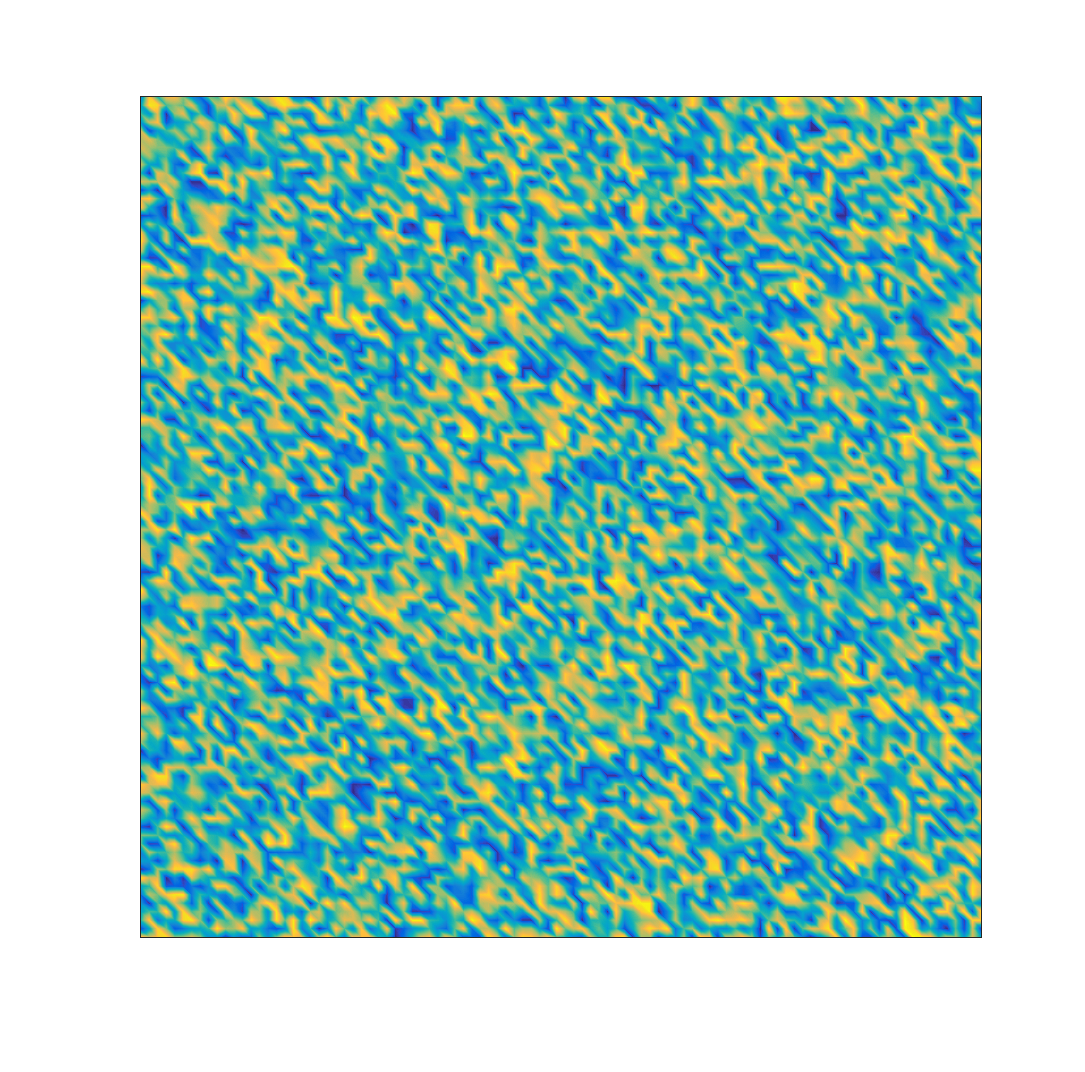
\includegraphics[width=1.84in]{13.pde1/spots-u-00.pdf}}
		\caption{Initial distribution}
		\label{fig:spots-u-00}
	\end{subfigure}
	\begin{subfigure}{0.31\textwidth}
		\centering
		\raisebox{0.055in}{\includegraphics[width=1.84in]{13.pde1/spots-u-20.pdf}}
		\caption{$t=20$}
		\label{fig:spots-u-20}
	\end{subfigure}
	\begin{subfigure}{0.35\textwidth}
		\centering
		\includegraphics[width=2in]{13.pde1/spots-u-100.pdf}
		\caption{$t=100$}
		\label{fig:spots-u-100}
	\end{subfigure}
\\
\vspace{0.2in}
	\begin{subfigure}{0.45\textwidth}
		\centering
		\includegraphics[width=2in]{13.pde1/spots-u.pdf}
		\caption{Steady state concentration of $X$}	
		\label{fig:spots-u}
	\end{subfigure}
	\begin{subfigure}{0.45\textwidth}
		\centering
		\includegraphics[width=2in]{13.pde1/spots-w.pdf}
		\caption{Steady state concentration of $Y$}	
		\label{fig:spots-w}
	\end{subfigure}
\caption{Time evolution of pattern formation.  Initially, the chemicals are randomly distributed. As time goes, a pattern begins to appear.  By $t=100$, a two dimensional crystal like structure is formed.  However, the pattern does not have a precise periodicity or symmetry yet. At $t=2000$, the system reaches a steady state.  The spot size is now identical and they form a hexagonal close-packing structure.  Parameter values are $a=2.5$, $b=5.0$, $D_u=0.2$, and $D_w=1.6$. Periodic boundary condition with $L=20$ is used. The discretization parameters are $h=1$, and $\Delta t=0.125\times 10^{-2}$.}
\label{fig:spots-evolution}
\end{figure}

The first chemical model to show oscillations and traveling waves was proposed
by Prigogine and Lefever\cite{prigogine68} in 1968.  The model is called the
"Brusselator"  because it was discovered in the city of Brussels.
The Brusselator system is the 
following sequence of reaction:
\begin{subequations}
\label{reactions} 
\begin{eqnarray}
A &\longrightarrow& X \\ 
B + X &\longrightarrow& Y + D \\
2X + Y &\longrightarrow& 3X \\ 
X &\longrightarrow& E
\end{eqnarray}
\end{subequations}
where the species $A$ and $B$ are sources whose concentration are kept
constant, and $D$ and $E$ are products which are extracted from the system at a
constant rate. The species $X$ and $Y$ are intermediate products. 
It is important to note that both $X$ and $Y$ are produced and
consumed during the sequence of reactions in such a way that $X$
produces $Y$ and $Y$ produces $X$.

When the reaction takes place in a well stirred container, the concentration of chemicals are uniform and does not depend on the position.  We have studied such a case in Section 4.4.1.  If the system is no stirred, the chemicals are not well mixed and the concentration becomes position-dependent.  The diffusion becomes the main mechanism of the mixing of the chemicals.  Then, the dynamics of the reaction is described by a pair of reaction-diffusion equations:
\begin{subequations}
\begin{eqnarray}
\pdv{t} u(\vb{r},t) &=& D_u \laplacian u(\vb{r},t) +a-(b+1)u(\vb{r},t) + u^2(\vb{r},t)\, w(\vb{r},t) \\
\pdv{t} w(\vb{r},t) &=& D_w \laplacian w(\vb{r},t) + b\, u(\vb{r},t) - u^2(\vb{r},t)\,w(\vb{r},t) 
\end{eqnarray}
\label{eq:reaction-diffusion-brussels}
\end{subequations}
where $u(\vb{r},t)$ and $w(\vb{r},t)$ are the concentration of chemicals $X$ and $Y$,  and $D_u$ and $D_w$ are their diffusion constants, respectively.  The parameters $a$ and $b$ remain constant both in space and time as before (see Section 4.4.1).

The reaction-diffusion equations (\ref{eq:reaction-diffusion-brussels}) has many different types of solution depending parameter values, initial conditions and boundary conditions, for examples, pattern formation, traveling wave, and spiral waves.

Equations \eqref{eq:reaction-diffusion-brussels} are essentially the diffusion equation with additional terms. Discretizing he time and space, we denote the two function as $u^k_{i,j} = u(t_k,x_i,y_j)$ and  $w^k_{i,j} = w(t_k,x_i,y_j)$.  Similarly to the 2-dimensional diffusion equation \eqref{eq:ftcs-2d}, the discrete version of the diffusion-reaction equations are
\begin{subequations}
    \begin{eqnarray}
 u^{k+1}_{i,j} &\approx& \rho^k_{i,j} + \frac{D_u \Delta t}{\Delta x^2} \left ( u^k_{i+1,j} + u^k_{i-1,j} - 2 u^k_{i,j} \right ) 
+ \frac{D_u \Delta t}{\Delta y^2} \left (u^k_{i,j+1} + u^k_{i,j-1} - 2 u^k_{i,j} \right ) \nonumber \\
 && + a-(b+1)u^k_{i,j}+ (u^k_{i,j})^2 w^k_{i,j} \\
  w^{k+1}_{i,j} &\approx& w^k_{i,j} + \frac{D_w \Delta t}{\Delta x^2} \left ( w^k_{i+1,j} + w^k_{i-1,j} - 2 w^k_{i,j} \right ) 
 + \frac{D_u \Delta t}{\Delta y^2} \left ( w^k_{i,j+1} + w^k_{i,j-1} - 2 w^k_{i,j} \right )
 \nonumber \\
  &&+ b u^k_{i,j} - (u^k_{i,j})^2 w^k_{i,j} 
    \end{eqnarray}
\end{subequations}\label{eq:brusselator-discrete}

Program \ref{prog:spots} implements Eq. (\ref{eq:brusselator-discrete}), with periodic boundary conditions in both directions.

We assume that the space is isotropic ($h=\Delta x = \Delta y$).
Initially, both $u$ and $w$ take independent random values between 0 and 1 at each point. 
Figure \ref{fig:spots-evolution} shows the time evolution of the concentration of $X$. Initially (Fig. \ref{fig:spots-u-00}) no simple pattern is seen but by time $t=20$ (Fig. \ref{fig:spots-u-20}) the high concentration regions is formed.  At $t=100$ (Fig. \ref{fig:spots-u-100}),  many circular spots with nearly the same radius are distributed with nearly equal distance between them.  The spots size is not exactly the same and they are not exactly aligned, it is clear that the spots are not randomly placed.  The reaction-diffusion system is organizing itself and forming a distinct order.
Figures \ref{fig:spots-u} and \ref{fig:spots-w} show the final steady state.  Each spot has the same size and they form hexagonal close packed structure like a two-dimensional crystal.

The patterns depend on the boundary conditions.  In the present example, the close-packing is formed due to the periodical boundary condition.  Other types of boundary conditions generates different patters.  It is also known that the same reaction-diffusion equation can generate spiral waves with appropriate boundary conditions and initial conditions. 


\newpage
\noindent
\section*{Program Lists}
\addcontentsline{toc}{section}{\protect\numberline{}Program Lists}

\noindent
\program
\label{prog:diffusion}
\footnotesize
\begin{verbatim}
%**************************************************************************
%*     Example 13.1                                                       *
%*     filename: ch13pr01.m                                               *
%*     program listing number: 13.1                                       *
%*                                                                        *
%*     This program solves a diffusion equation using the forward time    *
%*     centered space method.                                             *
%*                                                                        *
%*     Programed by Ryoichi Kawai for Computational Physics Course.       *
%*     Last modification:  02/15/2014.                                    *
%**************************************************************************
close all;
clear all;
% parameters
D=0.1; % diffusion constant
N=201; % number of grids
N1=(N-1)/2;
dx=0.1; % spacial step
R = 0.1; % D*dt/dx^2
dt=dx^2/D *R;  % time step

x=(-N1:N1)*dx; % spatial coordinates

M=10; % number of sample point.
tmax=10000; % total time steps
MS=tmax/M;

rho0=zeros(N,1);  % initial density profile
rho0(N1+1)=1.0/dx;

% allocate arrays
rho1=zeros(N,1);
rho=zeros(N,M);
t=zeros(M,1);

k=0;
for j=1:tmax
    rho1(1)=(1-R)*rho0(1)+R*rho0(2);  % left boundary
    rho1(N)=(1-R)*rho0(N)+R*rho0(N-1);  % right boundary
    for i=2:N-1
        rho1(i)=rho0(i)*(1-2*R)+R*(rho0(i+1)+rho0(i-1));
    end
    rho0=rho1;
    if mod(j,MS)==0  % record the results
        k=k+1;
        t(k)=j*dt;
        rho(:,k)=rho0(:);
    end
end

figure(1)
surf(t,(-N1:N1),rho)
    
figure(2)
for i=1:M
    plot(x,rho(:,i))
    hold on
end
hold off

figure(3)
f=1/sqrt(2*pi)*1/sqrt(2*D*t(2))*exp(-x.^2/(4*D*t(2))); % exact
plot(x,rho(:,2),'o',x,f)
legend('FTCS method','Exact')
\end{verbatim}
\normalsize

\noindent
\program
\label{prog:qm_tunneling}
\footnotesize
\begin{verbatim}
%**************************************************************************
%*     Example 13.2                                                       *
%*     filename: ch13pr02.m                                               *
%*     program listing number: 13.2                                       *
%*                                                                        *
%*     This program calculates quantum tunneling by solving a Shrodinger  *
%*     equation.  The Crank-Nicolson method is used.                      *
%*                                                                        *
%*     Programed by Ryoichi Kawai for Computational Physics Course.       *
%*     Last modification:  02/15/2014.                                    *
%**************************************************************************

clear all
close all

% system parameters
E=0.9;
k=sqrt(2*E);
a=5.0;
dt=0.1;

% control parameters
L=100;
h=0.05*min(a,2*pi/k);
N=2*round(L/h)+1;

% initial condition
x0=-L+5*a;
for j=1:N;
    x(j)=(j-(N+1)/2)*h;
    psi(j,1)=exp(-(x(j)-x0)^2/(2*a^2))*exp(i*k*x(j));
end
c=sum(abs(psi).^2)*h;
psi=psi/sqrt(c);

% construct matrix
A=zeros(N,N);
A(1,1)=complex(1,dt/h^2/2)/2;
A(1,2)=-i*dt/h^2/8;
for n=2:N-1
    A(n,n)=A(1,1);
    A(n,n-1)=A(1,2);
    A(n,n+1)=A(1,2);
end
A(N,N)=A(1,1);
A(N,N-1)=A(1,2);

% add potential barrier
V=complex(0,dt/4);
for n=(N+1)/2:(N+1)/2+5/h;
    A(n,n)=A(n,n)+V;
end

% solve Schrodinger equation.
for I=1:1000    
    chi = A\psi;
    psi = chi - psi;
    rho = abs(psi).^2;
    p=plot(x,rho); 
    set(p,'linewidth',2);
    hold on
    r=plot([0,0],[0,0.12],[5,5],[0,0.12],[0,5],[0.12,0.12]);
    set(r,'color','black');
    axis([-L L 0 0.12]);
    xlabel('$x$','interpreter','latex','fontsize',16)
ylabel('$|\psi(x)|^2$','interpreter','latex','fontsize',16)
hold off; drawnow;
end
    
% check the normalization
c=sum(abs(psi).^2)*h;
fprintf('Final Norm=%.6f\n',c)

% compute transmission/reflection probability
T=sum(abs(psi((N+1)/2+int32(5/h):N-1).^2))*h;
R=sum(abs(psi(1:(N-1)/2).^2))*h;
fprintf('Transmission Probability=%.6f\n',T)
fprintf('Reflection   Probability=%.6f\n',R)
\end{verbatim}
\normalsize

\noindent
\program
\label{prog:spots}
\footnotesize
\begin{verbatim}
%**************************************************************************
%*     Example 13.5.2                                                     *
%*     filename: ch13pr03.m                                               *
%*     program listing number: 13.3                                       *
%*                                                                        *
%*     This program solves a coupled reaction-diffusion systems based on  *
%*     the Brusselator model. The parameters are chosen to form spots.    *
%*                                                                        *
%*     Programed by Ryoichi Kawai for Computational Physics Course.       *
%*     Last modification:  02/15/2014.                                    *
%**************************************************************************
clear all
close all

% system parameters
a=2.5; b=5; % parameters for spots
Du=0.2; % diffusion constant for u
Dw=1.6; % duiffusion constant for w
L=20.0; % the size of the system (periodic boundary condition.

% control parameters
NL=100; % number of grid points
dx=L/NL; % step length
Du=Du/dx^2;
Dw=Dw/dx^2;
T=100; % total time (takes a long time to reach the final patttern)
dt=0.1/max(Du,Dw); % time step
NT=int32(T/dt);

% initial condition
u0=rand(NL,NL);
w0=rand(NL,NL);
pcolor(u0); axis equal tight; shading interp; drawnow;  

laplace_u=zeros(NL,NL);
laplace_w=zeros(NL,NL);

for k=1:NT
    t=(k-1)*dt;
    % Laplacian with periodic boundary
    laplace_u = circshift(u0,1,1)+circshift(u0,-1,1) ...
              + circshift(u0,1,2)+circshift(u0,-1,2) - 4*u0;
    laplace_w = circshift(w0,1,1)+circshift(w0,-1,1) ...
              + circshift(w0,1,2)+circshift(w0,-1,2) - 4*w0;
    % Euler step
    fu=a-(b+1)*u0+u0.^2.*w0+Du*laplace_u;
    fw=b*u0-u0.^2.*w0+Dw*laplace_w;
    u1=u0+fu*dt/2;
    w1=w0+fw*dt/2;
    
    % Laplacian at the mid time.
    laplace_u = circshift(u1,1,1)+circshift(u1,-1,1) ...
              + circshift(u1,1,2)+circshift(u1,-1,2) - 4*u1;
    laplace_w = circshift(w1,1,1)+circshift(w1,-1,1) ...
              + circshift(w1,1,2)+circshift(w1,-1,2) - 4*w1;

    % Runge-Kutta step
    fu=a-(b+1)*u1+u1.^2.*w1+Du*laplace_u;
    fw=b*u1-u1.^2.*w1+Dw*laplace_w;   
    u0=u0+fu*dt;
    w0=w0+fw*dt;
    
    pcolor(u0); axis equal tight; shading interp; drawnow;  
end
colorbar


figure(2)
pcolor(w0); axis equal tight; shading interp; drawnow;  
colorbar
\end{verbatim}
\normalsize

\vfill

\newpage
%\chapbibliography
\bibliographystyle{unsrt}
\bibliography{compphys}







%These three equations share a similar mathematical properties and can be solved in a similar numerical method.  However, since the wave function $\psi(x,t)$ is naturally complex, solving the Schr\"{o}dinger equation is more comlicated than the other two equations.  Note also that the Sch\"{o}dinger equation is not a wave equation of hyperbolic form although $\psi(x,t)$ is called wave function.




%The simple examples (\ref{eq:diffusion})--(\ref{eq:schrodinger}) are essential to understand the parabolic PDE.  However, we can solve them analytically. We need numerical methods for parabolic PDEs with additional terms.  An extension of the diffusion equation (\ref{eq:diffusion} is the
%Fokker-Plank equation
%\begin{equation}
%	\pdv{t} \rho(x,t) = \left [ -\pdv{x} F(x,t) + \pdv[2]{}{x} D(x,t) \right ] \rho(x,t).
%\end{equation}
%which determines the time-evolution of Brownian particles with external forces.  Note that the diffusion constant can depend on %the coordinates.  A more complicated system involves multiple species whose density is given by a vector function %$\vb*{\rho}(x,t) = [\rho_1(x,t), \cdots, \rho_N(x,t)]$.  In addition to diffusion, the species can undergo chemical reaction %between them.  The system is described by a reaction-diffusion equation
%\begin{equation}
%	\pdv{t} \vb*{\rho}(x,t) = \pdv[2]{}{x} \vb{D} \vdot \vb*{\rho}(x,t) + \vb{R}[\vb*{\rho}(x,t)]
%\end{equation}
%where $\vb{D}$ is a vector whose component $D_i$ is the diffusion constant of the $i$-th species.  $\vb{R}()$ is a vector function which defines the chemical reactions.


%The dynamics of a quantum particle in a potential field $U(x)$ is determined by Schr\"{o}dinger equation
%\begin{equation}
%	i \hbar \pdv{t} \psi(x,t) = \left [ -\frac{\hbar^2}{2m} \pdv[2]{}{x} + U(x) \right ] \psi(x)
%\end{equation}
%which is also a kind of parabolic PDE.